\section{Introduction}
% Fix citations

In this chapter, we perform simulations to gauge the effectiveness of the DSD metric in improving the prediction of labels on data for scale-free networks [CITE], Watts-Strogatz small-world networks [CITE], and some networks we constructed with hypotheses of how the DSD metric should affect classification on them. We compare the DSD metric with the shortest-path distance metric, which is used in some modern approaches of label prediction, such as k-nearest neighbor classifiers [CITE] and laplacian eigenmaps [CITE]. Although several methods for measuring distance or similarity among vertices in a network use the shortest-path distance in the network, the DSD metric is designed to capture distinctions in similarity not captured by the shortest-path distance alone. Thus, we compare effectiveness of the DSD metric and the shortest-path distance metric. We expect the shortest path distance metric to be less effective than the DSD metric for networks with high clustering coefficients or networks with a small diameter, such as small-world networks. Any vertex in such a network is close to any other node in the network, making the shortest-path distance of any two nodes close. We also expect the DSD metric to be more effective on networks with hub vertices, since these vertices tend to make the network highly connected with a small diameter.

In the same way, we compare the DSD metric with centrality and node influence measures, which are designed to capture the influence of vertices in a graph. Centrality identifies the most important vertices in a graph using various methods such as network flows and walks on the graph [CITE]. Various centrality indices are defined using different properties of vertices that capture different distinctions in similarity than the DSD metric. We study several types of centralities including degree centrality, eigenvector centrality, and dissimilarity based centrality measures. These notions of centrality are more related to the DSD metric than the shortest-paths metric, so we expect that they will be similarly effective in predicting labels.

We hope to reveal properties of graphs that allow the DSD metric to be more effective at classification.

\section{Label Prediction Methods}
In this section, we discuss several prediction methods that we use for our simulations in chapter 5. These prediction methods can use any graph metric to predict labels. Thus, for a simulation, we test different metrics using the same prediction method and compare results. This allows us to study the effectiveness of various metrics in improving the accuracy of a certain prediction method. In short, the prediction method is not dependent on any metric, but predictive results may change for different metrics. The following prediction methods assume that a graph $G=(V,E)$ is given on which prediction is to be done.

\subsection{Majority Voting Algorithm}
% Weighting by dist? Metric?
Cao et al. ~\cite{10.1371/journal.pone.0076339} mentions a simple prediction method called the neighborhood majority voting algorithm. We considered two implementations of this algorithm. One implementation considers each vertex $v \epsilon V$ and all neighbors of $v$ within an $\varepsilon$ distance from $v$ (a ball of radius $\varepsilon$). The $\varepsilon$ distance depends on the metric under consideration, and may be changed as a parameter. In an unweighted scheme, each neighbor within the ball of radius $\varepsilon$ votes equally for their own label. In a weighted scheme, each neighbor gets a vote proportional to the reciprocal of their distance to the vertex $v$ in consideration. The other implementation of this algorithm considers each vertex $v \epsilon V$ and the $k$-nearest neighbors of $v$. Voting is done similarly in both an unweighted and weighted scheme.


\section{Complete Components}
In this section, we construct of a family of graphs with an intuitive initial labeling of vertices. We then run simulations on this graph to determine the difference in effectiveness between the DSD metric and the shortest path metric on this family of graphs.

\subsection{Graph Construction}
We construct a graph starting with the disjoint union of two $n$-complete graphs $G_{1} = (V_{1},E_{1})$, $G_{2} = (V_{2},E_{2})$. An $n$-complete graph is defined as a graph with $n$ vertices in which every pair of vertices is connected by an edge. All vertices from $G_{1}$ were labeled red, and all vertices from $G_{2}$ were labeled blue. We call the disjoint union of $G_{1}$ and $G_{2}$ as the graph $G = (V,E)$, with vertex set $V = V_{1} \cup V_{2}$ and edge set $E = E_{1} \cup E_{2}$. In order to introduce noise in $G$, we remove edges from the current edge set with a probability $q$, and add edges having one end in $V_{1}$ and the other end in $V_{2}$ with a probability $p$. Lastly, we take the largest connected component of the resulting graph and set it as our graph $G$.

\subsection{Data Collection}
We studied the classification problem on the complete components graph. After constructing the complete components graph $G$ with parameters $n$, $p$ and $q$ described in the section above, we censored a proportion $censorP$ of the labels in $G$. We then used the weighted majority voting algorithm using $k$-nearest neighbors with respect to both the shortest path distance metric and the DSD metric to predict labels. To make sure the prediction accuracy was robust, we ran this process several times and took the average of the resulting prediction accuracies. We adding a parameter called $avgRuns$ to describe how many times we would run this process for the average prediction accuracy.

To test the behavior of the prediction accuracy with respect to different parameters of the complete components graph, we ran several simulations using varying parameter inputs. The parameter $n$, the size of one complete graph used in the construction of the complete components graph, was set to $250$. A constant value for this parameter sufficiently large would allow us to observe differences in prediction accuracy and changing this parameter would not affect the prediction accuracy. The parameter for the average number of runs for calculating prediction accuracy, $avgRuns$ was also set to a constant value of $10$, since this parameter would not affect the prediction accuracy. The parameter for the proportion of the graph labels to censor, $censorP$, was also set to a constant $0.3$ because this would not affect the prediction accuracy, as shown in figure \ref{fig:censor_param}.

% Hard to read
\begin{figure}[h!]
\centering
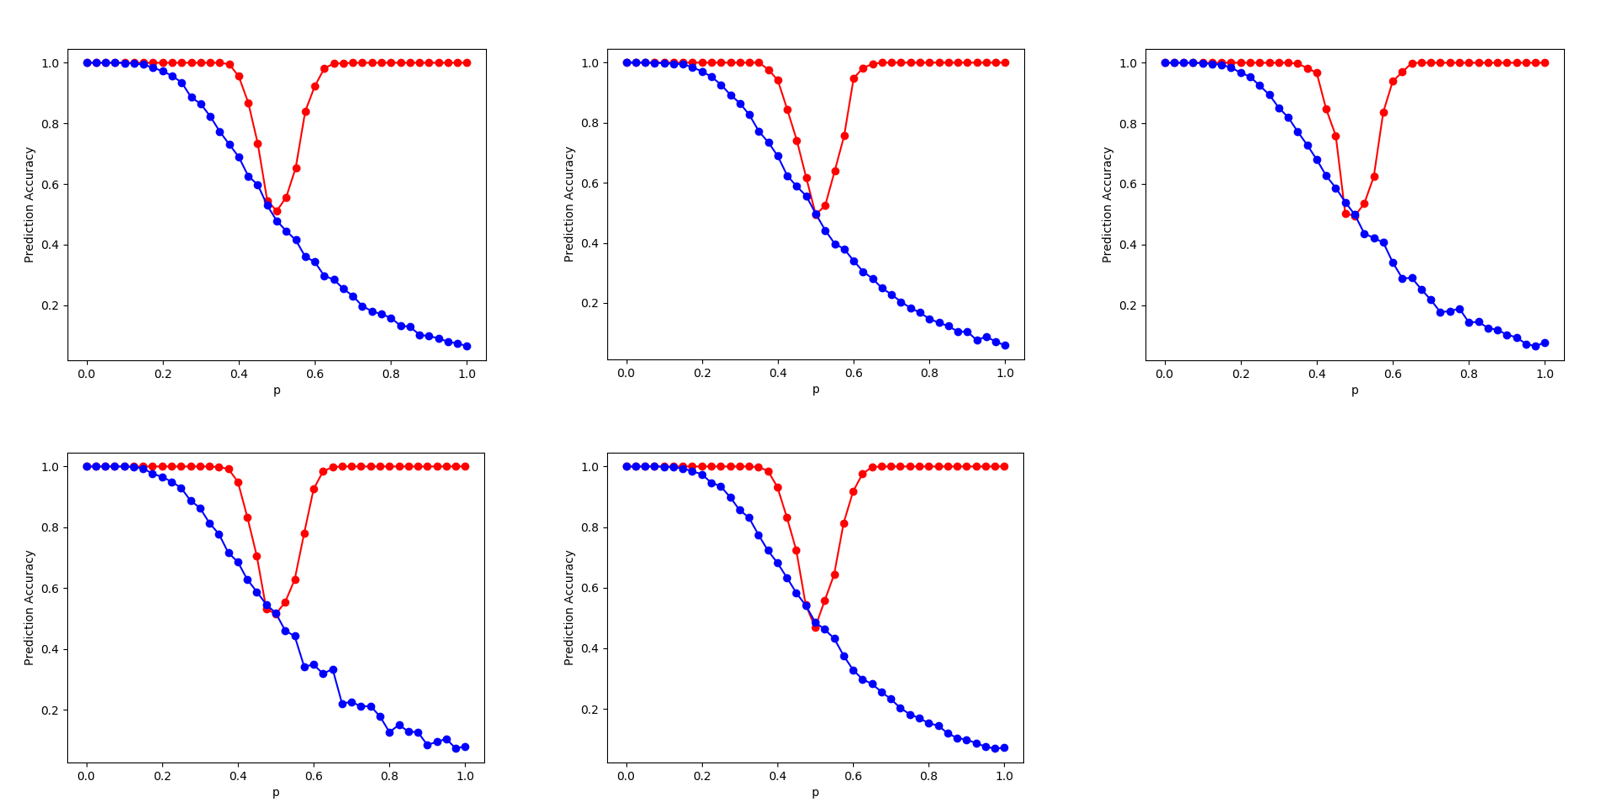
\includegraphics[width=1.0\textwidth]{censor_param.png}
\caption{Plots showing that the censoring parameter $censorP$ has no affect on prediction accuracy. $n = 250$, $avgRuns = 10$, $q = 0.5$, $p$ goes from $0$ to $1$ in intervals of $0.025$, and $censorP$ goes from $0.1$ to $0.9$ in intervals of $0.2$.}
\label{fig:censor_param}
\end{figure}


The parameters that we varied in our simulations for the complete components graphs were $p$ and $q$. Figure \ref{fig:cc_p_q} shows a plot of prediction accuracies for a fixed $q = 0.5$ and $p$ going from $0$ to $1$ in intervals of $0.025$. Figure \ref{fig:cc_q_p} shows a plot of prediction accuracies for a fixed $p = 0.5$ and $q$ going from $0$ to $1$ in intervals of $0.025$.

\begin{figure}[h!]
\centering
\includegraphics[width=0.75\textwidth]{{cc_p_n250_q0.5_c0.1_avg10_mv-k20}.png}
\caption{A plot showing the change in prediction accuracy for a fixed $q = 0.5$ and $p$ from $0$ to $1$ in intervals of $0.025$.}
\label{fig:cc_p_q}
\end{figure}

\begin{figure}[h!]
\centering
\includegraphics[width=0.75\textwidth]{{cc_q_n250_p0.5_c0.1_avg10_mv-k20}.png}
\caption{A plot showing the change in prediction accuracy for a fixed $p = 0.5$ and $q$ from $0$ to $1$ in intervals of $0.025$.}
\label{fig:cc_q_p}
\end{figure}


\subsection{Analysis}
We can expect prediction using the DSD metric to do significantly better than prediction using the shortest path distance metric. This can be seen from Figure \ref{fig:cc_p_q} and Figure \ref{fig:cc_q_p}, and can also be shown using expected values.

Using the parameters from the simulation run shown in Figure \ref{fig:cc_p_q}, we get that for an arbitrary vertex $v$, $deg_{same}(v) = (1-0.5)(250-1) = 124.5$. Since $deg_{diff} = 250p$, we know that $deg_{diff}$ will increase or decrease proportional to the change in $p$. For values of $p$ between $0$ and $0.5$, we know that $deg_{same} > deg_{diff}$. It is clear that the shortest path distance metric should predict with a fairly high accuracy for $p$ close to $0$, but should predict no better than a random guess for $p$ close to $0.5$. The prediction accuracy of the shortest path distance only becomes worse for $p$ greater than $0.5$, since $deg_{same} < deg_{diff}$.